% Chapter Template

\chapter{Microwave Resonators} % Main chapter title

\label{Chapter2} % Change X to a consecutive number; for referencing this chapter elsewhere, use \ref{ChapterX}

%----------------------------------------------------------------------------------------
%	SECTION 1
%----------------------------------------------------------------------------------------

\section{Theory}

In most low frequency AC circuits, we are used to transmitting the signal in 2 conductors (or wires). At these frequencies, the wavelength of the signal is very large compared to the length of the conductors, so we assume that the signal is the same as the generator signal at all points in the conductors. In reality, there will be a small phase shift and an amplitude loss between the signal at the signal generator and the other end of the "wires". This phase shift, along with other phenomena can be easily observed at high frequencies.

At high frequencies, the geometry and properties of the material plays an important role in the transmission. The replacement for what we knew as just "wires" are called \textit{Transmission Lines} or \textit{Waveguides}.

%-----------------------------------
%	SUBSECTION 1
%-----------------------------------
\subsection{Waveguides}

There are many different types of waveguides. Some of them are shown in Fig. \ref{fig:waveguides}. The case we will be dealing with in this thesis pertains to rectangular waveguide.

\begin{figure}
\centering
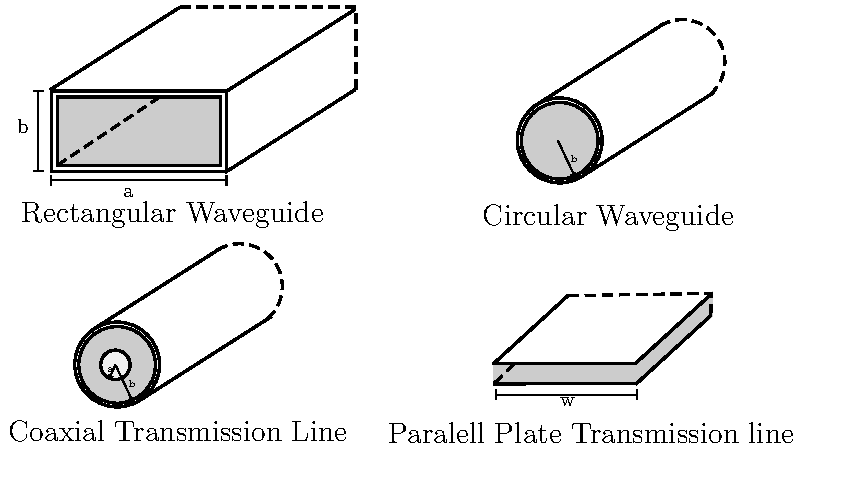
\includegraphics{Figures/Waveguides}
\decoRule
\caption[Waveguide Types]{Types of Waveguides and Transmission Lines}
\label{fig:waveguides}
\end{figure}

\subsubsection{General Waveguide}

Consider a general cross-section of a dielectric surrounded by conductor (can have one more conductor in the dielectric) which continues infinitely along the $z$ axis. We can write down the electric and magnetic fields in the dielectric in phasor domain. We assume that the wave propagates in the $z$-axis and has an $e^{j\omega t}$ dependence.

\begin{equation}
\bar{E}(x,y,z)=[\hat{x}e_x(x,y)+\hat{y}e_y(x,y)+\hat{z}e_z(x,y)]e^{-j\beta z}
\label{eqn:electric field general}
\end{equation}

\begin{equation}
\bar{H}(x,y,z)=[\hat{x}h_x(x,y)+\hat{y}h_y(x,y)+\hat{z}h_z(x,y)]e^{-j\beta z}
\label{eqn:magnetic field general}
\end{equation}

Here $\beta$, the propagation constant, is a real number. $j\beta$ must be replaced with $\gamma=\alpha+j\beta$ if attenuation is also to be considered.

Then, if the dielectric in the waveguide has no charges or currents, we can write Maxwell's equations as

\begin{subequations}
\label{eqn:maxwell curl}
\begin{align}
\nabla \times \bar{E}& =-j\omega \mu \bar{H}
\label{eqn:maxwell electric curl}\\
\nabla \times \bar{H}& =j\omega \epsilon \bar{E}
\label{eqn:maxwell magnetic curl}
\end{align}
\end{subequations}
Taking the curl of \ref{eqn:maxwell electric curl} gives
\begin{equation}
\nabla \times \nabla \times \bar{E}=-j\omega\mu \nabla \times \bar{H}=\omega^2 \mu\epsilon \bar{E}
\end{equation}
Using the vector identity $\nabla\times\nabla\times\bar{A}=\nabla(\nabla .\bar{A})-\nabla^2 \bar{A}$ and $\nabla .\bar{E}=0$ for a region with no sources ($\rho=0$) we get
\begin{equation}
\nabla^2 \bar{E}+\omega^2\mu\epsilon\bar{E}=0
\end{equation}

Similarly, we can also take the curl of \ref{eqn:maxwell magnetic curl} to get
\begin{equation}
\nabla^2 \bar{H}+\omega^2\mu\epsilon\bar{H}=0
\end{equation}

For a $z$ dependence of $e^{-j\beta z}$, $E_z$ and $H_z$ can be written as
\begin{equation}
\left(\frac{\partial^2}{\partial x^2}+\frac{\partial^2}{\partial y^2}+k^2-\beta^2\right)E_z=0
\label{eqn:diff Ez}
\end{equation}
\begin{equation}
\left(\frac{\partial^2}{\partial x^2}+\frac{\partial^2}{\partial y^2}+k^2-\beta^2\right)H_z=0
\label{eqn:diff Hz}
\end{equation}
since $\frac{\partial^2}{\partial z^2}\left(Ae^{-j\beta z}\right)=-\beta Ae^{-j\beta z}$.
Let us define $k_c^2=k^2-\beta^2$ for convenience.

After writing down the 6 equations that arise from \ref{eqn:maxwell curl} and eliminating variables, we can write $E_x$, $E_y$, $H_x$, $H_y$ in terms of $E_z$ and $H_z$ as follows

\begin{subequations}
\label{eqn:general fields}
\begin{align}
E_x& =\frac{-j}{k_c^2}\left(\beta\frac{\partial E_z}{\partial x} + \omega\mu\frac{\partial H_z}{\partial y}\right)
\label{eqn:Ex}
\\
E_y& =\frac{j}{k_c^2}\left(-\beta\frac{\partial E_z}{\partial y}+ \omega\mu\frac{\partial H_z}{\partial x}\right)
\label{eqn:Ey}
\\
H_x& =\frac{j}{k_c^2}\left(\omega\epsilon\frac{\partial E_z}{\partial y}-\beta\frac{\partial H_z}{\partial x}\right)
\label{eqn:Hx}
\\
H_y& =\frac{-j}{k_c^2}\left(\omega\epsilon\frac{\partial E_z}{\partial x}+\beta\frac{\partial H_z}{\partial y}\right)
\label{eqn:Hy}
\end{align}
\end{subequations}
where
\begin{equation}
k_c^2=k^2-\beta^2
\label{eqn:kc definition}
\end{equation}
\begin{equation}
k=\omega \sqrt{\mu\epsilon}=2\pi/\lambda
\label{eqn:k=2pi/lambda}
\end{equation}

These equations (\ref{eqn:diff Ez}, \ref{eqn:diff Hz} and \ref{eqn:general fields}) can be used for any waveguide. There are three types of waves that are possible in waveguides: Transverse Electric and Magnetic mode (TEM), Transverse Electric mode (TE) and Transverse Magnetic mode (TM).

\begin{enumerate}
\item \textbf{TEM modes}

In this mode $E_z=H_z=0$, meaning there are only transverse fields.
\item \textbf{TE modes}

In this mode $E_z=0$, meaning there are only transverse electric fields.
\item \textbf{TM modes}

In this mode $H_z=0$, meaning there are only transverse magnetic fields.
\end{enumerate}

\subsubsection{Rectangular Waveguide}

Let us now concentrate on the fields in a rectangular waveguide. It can be shown that in the TEM mode, fields in the dielectric follow the same rules as electrostatics \cite{Pozar2009}. In a single conductor waveguide like the rectangular waveguide, the electrostatic potential is zero (or constant) which means that $E=0$ and $H=0$. This means we can only have TE and TM modes in the rectangular waveguide (or any single conductor waveguide).

\begin{enumerate}
\item \textbf{TE modes}

Equation \ref{eqn:diff Hz} has been rewritten below with $k^2-\beta^2$ replaced with $k_c$ and divided by $e^{-j\beta z}$.
\begin{equation}
\left(\frac{\partial^2}{\partial x^2}+\frac{\partial^2}{\partial y^2}+k_c^2\right)h_z=0
\label{eqn:hz diff}
\end{equation}
Here, $H_z(x,y,z)=h_z(x,y)e^{-j\beta z}$.

We can solve \ref{eqn:hz diff} using separation of variables. We assume
\begin{equation}
h_z(x,y)=F(x)G(y)
\end{equation}
Substituting this into \ref{eqn:hz diff} gives
\begin{equation}
\frac{1}{F}\frac{d^2F}{dx^2}+\frac{1}{G}\frac{d^2G}{dy^2}+k_c^2=0
\end{equation}
Now, since each term is independent of each other, each term must be a constant. We define the first term to be $k_x^2$ and the second term to be $k_y^2$ to get 
\begin{equation}
k_x^2+k_y^2+k_c^2=0
\end{equation}
Then we get 2 ordinary differential equations
\begin{subequations}
\label{eqn:separation}
\begin{align}
\frac{d^2F}{dx^2}+k_xF& =0\\
\frac{d^2G}{dy^2}+k_yG& =0
\end{align}
\end{subequations}
The general solution to \ref{eqn:separation} is
\begin{subequations}
\begin{align}
F& =A\cos(k_xx)+B\sin(k_xx)\\
G& =C\cos(k_yy)+D\sin(k_yy)
\end{align}
\end{subequations}
Which gives
\begin{equation}
h_z =(A\cos(k_xx)+B\sin(k_xx))(C\cos(k_yy)+D\sin(k_yy))
\label{eqn:hz general}
\end{equation}

Since the boundary conditions we have are that the tangential electric field at the conductor is zero, i.e.
\begin{subequations}
\begin{align}
e_x(x,y)& =0 & \text{ at } y=0 \text{ and } y=b
\label{eqn:ex boundary}\\
e_y(x,y)& =0 & \text{ at } x=0 \text{ and } x=a
\label{eqn:ey boundary}
\end{align}
\end{subequations}

Substituting $E_z=0$ in \ref{eqn:general fields}, we get
\begin{subequations}
\label{eqn:TE transverse diff}
\begin{align}
E_x& =\frac{-j\omega\mu}{k_c^2}\frac{\partial H_z}{\partial y}\\
E_y& =\frac{-j\omega\mu}{k_c^2}\frac{\partial H_z}{\partial x}\\
H_x& =\frac{-j\beta}{k_c^2}\frac{\partial H_z}{\partial x}\\
H_y& =\frac{-j\beta}{k_c^2}\frac{\partial H_z}{\partial y}
\end{align}
\end{subequations}

Now substituting $h_z(x,y)$ from \ref{eqn:hz general} we get the following electric fields
\begin{subequations}
\begin{align}
e_x& =\frac{-j\omega\mu}{k_c^2}k_y(A\cos(k_xx)+B\sin(k_xx))(-C\sin(k_yy)+D\cos(k_yy))\\
e_y& =\frac{j\omega\mu}{k_c^2}k_x(-A\sin(k_xx)+B\cos(k_xx))(C\cos(k_yy)+D\sin(k_yy))
\end{align}
\end{subequations}
Now applying the boundary conditions,\\
from \ref{eqn:ex boundary} we get $D=0$ and $k_y=n\pi/b$ for $n={0,1,2\ldots}$,\\
and from \ref{eqn:ey boundary} we get $B=0$ and $k_x=m\pi/a$ for $m={0,1,2\ldots}$.\\
From this we know the propagation constant is
\begin{equation}
\beta = \sqrt{k^2-k_c^2}=\sqrt{k^2-\left(\frac{m\pi}{a}\right)^2-\left(\frac{n\pi}{b}\right)^2}
\end{equation}
Since $\beta$ is real, we now have a cut-off frequency for which $k^2>k_c^2$. This means that if $a>b$, there will be a range of frequencies for which $TE_{mn}=TE_{10}$ will have propagation but $TE_{01}$ will not.

The final solution for $H_z$ is
\begin{equation}
H_z(x,y,z)=A_{mn}\cos\left(\frac{m\pi x}{a}\right)\cos\left(\frac{n\pi y}{b}\right)e^{-j\beta z}
\label{Hz final}
\end{equation}
where $A_{mn}=AC$.

Now we can find $E_x, E_y, H_x$ and $H_y$ using \ref{eqn:TE transverse diff}
\begin{subequations}
\label{eqn:TE transverse fields}
\begin{align}
E_x(x,y,z)& =\frac{j\omega\mu n\pi}{k_c^2b}A_{mn}\cos\left(\frac{m\pi x}{a}\right)\sin\left(\frac{n\pi y}{b}\right)e^{-j\beta z}\\
E_y(x,y,z)& =\frac{-j\omega\mu m\pi}{k_c^2a}A_{mn}\sin\left(\frac{m\pi x}{a}\right)\cos\left(\frac{n\pi y}{b}\right)e^{-j\beta z}\\
H_x(x,y,z)& =\frac{j\beta m\pi}{k_c^2a}A_{mn}\sin\left(\frac{m\pi x}{a}\right)\cos\left(\frac{n\pi y}{b}\right)e^{-j\beta z}\\
H_y(x,y,z)& =\frac{j\beta n\pi}{k_c^2b}A_{mn}\cos\left(\frac{m\pi x}{a}\right)\sin\left(\frac{n\pi y}{b}\right)e^{-j\beta z}
\end{align}
\end{subequations}

These equations are only for a wave propagating in one direction. The total electric field well have another term for the fields with a different constant. We can replace $A_{mn}$ with $A_{mn}^+$ (for $+z$ direction propagation) and $A_{mn}^-$ (for $-z$ direction propagation). Then the transverse fields for each mode ($m,n$) would take the form
\begin{subequations}
\begin{align}
\bar{E}_t(x,y,z)& =[\hat{x}e_x(x,y)+\hat{y}e_y(x,y)](A^+e^{-j\beta z}+A^-e^{+j\beta z})\\
\bar{H}_t(x,y,z)& =[\hat{x}h_x(x,y)+\hat{y}h_y(x,y)](A^+e^{-j\beta z}-A^-e^{+j\beta z})
\end{align}
\end{subequations}
The negative sign for $A^-$ in the magnetic field is to ensure that the direction of propagation given by $\bar{E}_t\times\bar{H}_t$ is opposite.

\item \textbf{TM modes}

The TM modes can be derived in exactly the same way except that the boundary conditions will apply directly to $E_z$ this time.

The fields for the TM modes are
\begin{subequations}
\begin{align}
E_z(x,y,z)& =B_{mn}\sin\left(\frac{m\pi x}{a}\right)\sin\left(\frac{n\pi y}{b}\right)e^{-j\beta z}\\
E_x(x,y,z)& =\frac{-j\beta m\pi}{k_c^2a}B_{mn}\cos\left(\frac{m\pi x}{a}\right)\sin\left(\frac{n\pi y}{b}\right)e^{-j\beta z}\\
E_y(x,y,z)& =\frac{-j\beta n\pi}{k_c^2b}B_{mn}\sin\left(\frac{m\pi x}{a}\right)\cos\left(\frac{n\pi y}{b}\right)e^{-j\beta z}\\
H_x(x,y,z)& =\frac{j\omega\epsilon n\pi}{k_c^2b}B_{mn}\sin\left(\frac{m\pi x}{a}\right)\cos\left(\frac{n\pi y}{b}\right)e^{-j\beta z}\\
H_y(x,y,z)& =\frac{-j\omega
\epsilon m\pi}{k_c^2a}B_{mn}\cos\left(\frac{m\pi x}{a}\right)\sin\left(\frac{n\pi y}{b}\right)e^{-j\beta z}
\end{align}
\end{subequations}

Notice that if $m$ or $n$ is zero, then the fields all go to zero. So there is no $TM_{10}$ or $TM_{01}$ mode.

The propagation constant $\beta$ is
\begin{equation}
\beta = \sqrt{k^2-k_c^2}=\sqrt{k^2-\left(\frac{m\pi}{a}\right)^2-\left(\frac{n\pi}{b}\right)^2}
\end{equation}

This means the cut-off frequencies are the same for the TE and TM modes. Now we can see that there is a range of frequencies where only the $TE_{10}$ mode will propagate. This feature of waveguides is used extensively to avoid complications of other modes interfering with the signal.
\end{enumerate}


%-----------------------------------
%	SUBSECTION 2
%-----------------------------------

\subsection{Rectangular Waveguide Resonators}

Now that we know what modes and what frequencies can propagate in a rectangular waveguide, we can convert the waveguide into a resonator by walling the 2 infinitely open faces with conducting surfaces to make a cuboid filled with dielectric. This structure is often called a rectangular cavity.\\

We can use the equations we derived in the previous section for fields and the propagation constant to see what effects the new conducting walls will have.

We can start by writing down the transverse electric field ($E_t = \hat{x}E_x+\hat{y}E_y$)
\begin{equation}
\bar{E}_t=\bar{e}(x,y)(A^+e^{-j\beta z}+A^-e^{+j\beta z})
\label{eqn:Et start}
\end{equation}
where $\bar{e}(x,y)$ is the variation in the transverse fields.
\begin{equation}
\beta = \sqrt{k^2-\left(\frac{m \pi}{a}\right)^2-\left(\frac{n \pi}{b}\right)^2}
\end{equation}

The new boundary conditions added now are that $E_t=0$ at the 2 new walls, $z=0$ and $z=d$.\\
For $z=0$, \ref{eqn:Et start} gives 
\begin{equation}
A^+=-A^-
\end{equation}.\\
For $z=d$, \ref{eqn:Et start} gives
\begin{equation}
-\bar{e}(x,y)A^+2j\sin(\beta_{mn}d)=0
\end{equation}
The solution to this equation (other than $A^+=0$) is
\begin{equation}
\beta_{mn}=\frac{l\pi}{d} \text{ where } l=1,2,3\ldots
\end{equation}
This means that, given a frequency, propagation (or in this case resonance) occurs only for particular lengths. $\beta^2=k^2-k_c^2$ can be rearranged to get
\begin{equation}
k_{mnl}=\sqrt{\left(\frac{m \pi}{a}\right)^2+\left(\frac{n \pi}{b}\right)^2+\left(\frac{l \pi}{d}\right)^2}
\end{equation}
The resonant frequency is given by
\begin{equation}
f_{mnl}=\frac{ck_{mnl}}{2\pi\sqrt{\mu_r\epsilon_r}}=\frac{c}{2\pi\sqrt{\mu_r\epsilon_r}}\sqrt{\left(\frac{m \pi}{a}\right)^2+\left(\frac{n \pi}{b}\right)^2+\left(\frac{l \pi}{d}\right)^2}
\end{equation}

Now let us restrict ourselves to the $TE_{10l}$ mode of the resonator. Since $A^-=-A^+$, the fields for this mode are
\begin{subequations}
\label{eqn:TE10l fields}
\begin{align}
E_y(x,y,z)& =A^+\sin\left(\frac{\pi x}{a}\right)(e^{-j\beta z}-e^{+j\beta z})\\
H_x(x,y,z)& =\frac{-A^+}{Z_{TE}}\sin\left(\frac{\pi x}{a}\right)(e^{-j\beta z}+e^{+j\beta z})\\
H_z(x,y,z)& =\frac{j\pi A^+}{k\eta a}\cos\left(\frac{\pi x}{a}\right)(e^{-j\beta z}-e^{+j\beta z})
\end{align}
\end{subequations}
where
\begin{subequations}
\begin{align*}
A^+& =\frac{-j\omega\mu m\pi}{k_c^2a}\\
Z_{TE}& =\frac{\omega\mu}{\beta}& 
k& =\omega\sqrt{\mu\epsilon}\\
k_c^2& =\sqrt{\frac{\pi}{a}}& 
\eta& =\sqrt{\frac{\mu}{\epsilon}}
\end{align*}
\end{subequations}

Using $-2jA^+=E_0$, we can simplify the above equations to
\begin{subequations}
\begin{align}
E_y(x,y,z)& =E_0\sin\left(\frac{\pi x}{a}\right)\sin\left(\frac{l\pi z}{d}\right)\\
H_x(x,y,z)& =\frac{-jE_0}{Z_{TE}}\sin\left(\frac{\pi x}{a}\right)\cos\left(\frac{l\pi z}{d}\right)\\
H_z(x,y,z)& =\frac{j\pi E_0}{k\eta a}\cos\left(\frac{\pi x}{a}\right)\sin\left(\frac{l\pi z}{d}\right)
\end{align}
\end{subequations}

We can now calculate the \textit{quality factor} $Q$ by calculating the energy stored and power lost in the resonator.
The stored electric energy is, from \cite{Pozar2009}
\begin{equation}
W_e=\frac{\epsilon}{4}\int_V E_yE_y^*dv = \frac{\epsilon abd}{16}E_0^2
\end{equation}
and the stored magnetic energy is
\begin{align}
\begin{split}
W_m&=\frac{\mu}{4}\int_V (H_xH_x^*+H_zH_z^*)dv\\
&= \frac{\mu abd}{16}E_0^2\left(\frac{1}{Z_{TE}^2}+\frac{\pi^2}{k^2\eta^2a^2}\right)\\
&=\frac{\mu abd}{16}E_0^2\left(\frac{\beta^2+(\pi/a)^2}{k^2\eta^2}\right)\\
&=\frac{\mu abd}{16}E_0^2\left(\frac{1}{\eta^2}\right)\\
&=\frac{\epsilon abd}{16}E_0^2
\end{split}
\end{align}
Note that $W_e=W_m$ at resonance.

The power lost by the conducting walls is
\begin{equation}
P_c=\frac{R_s}{2}\int_{walls} |H_t|^2ds
\end{equation}
where $R_s=\sqrt{\omega\mu_0/(2\sigma)}$ is the surface resistivity and $H_t$ is the tangential magnetic field at the walls. This gives
\begin{equation}
P_c=\frac{R_sE_0^2\lambda^2}{8\eta^2}\left(\frac{l^2ab}{d^2}+\frac{bd}{a^2}+\frac{l^2a}{2d}+\frac{d}{2a}\right)
\end{equation}

The power dissipated from the lossy dielectric with $\epsilon = \epsilon'-j\epsilon''$ is
\begin{equation}
P_d = \frac{1}{2}\int_V\bar{J}.\bar{E}=\frac{\omega\epsilon''}{2}\int_V|\bar{E}|^2dv=\frac{abd\omega\epsilon''|E_0|^2}{8}
\end{equation}

The quality factor $Q$ is defined as
\begin{align}
\begin{split}
Q&=\omega\frac{\text{average energy stored}}{\text{average power loss}}\\
&=\omega\frac{W_e+W_m}{P_{loss}}\\
&=\omega\frac{2W_e}{P_c+P_d}
\end{split}
\end{align}

\subsection{Coupling to an External Circuit}

A resonator is useless if we cannot communicate with it in some way. There are many ways of interacting with a resonator. In the experiments to follow, the rectangular cavity resonator will be coupled to and external circuit through a probe of height $h$ inserted at the $y=0$ wall at $x=a/4$ and $z=0$. A figure of the probe inserted in the rectangular cavity is shown in Fig.\ref{fig:Probe}.

\begin{figure}
\centering
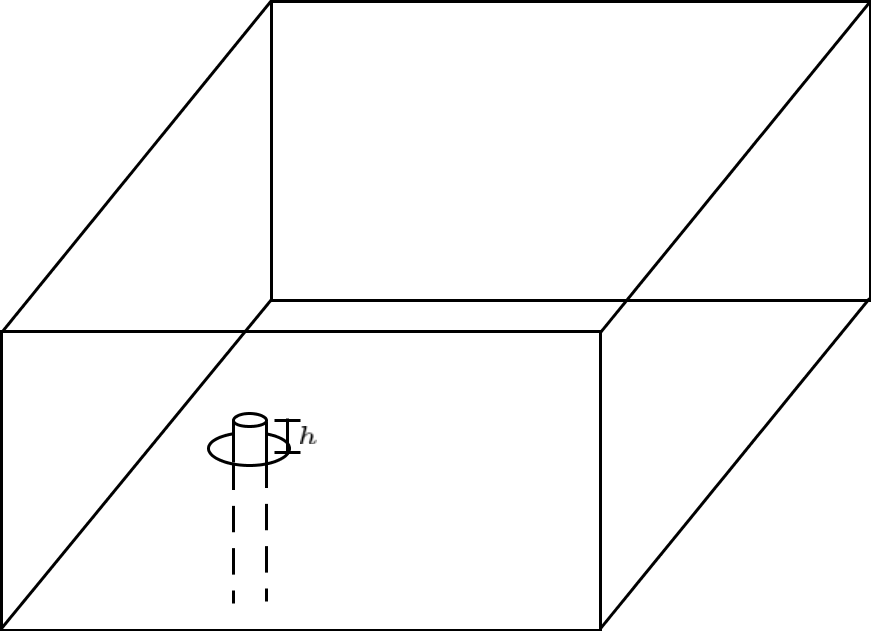
\includegraphics[width=250px]{Figures/probe}
\decoRule
\caption[Probe in resonator]{The probe is inserted up to a height $h$ into the cavity. The other end of the probe is a coaxial cable whose outer terminal is connected to the cavity.}
\label{fig:Probe}
\end{figure}

The equivalent circuit, shown in Fig.\ref{fig:external circuit} for this setup would be a paralell RLC circuit capacitively coupled to the measurement device, which in this case is a VNA (Vector Network Analyzer).

\begin{figure}
\centering
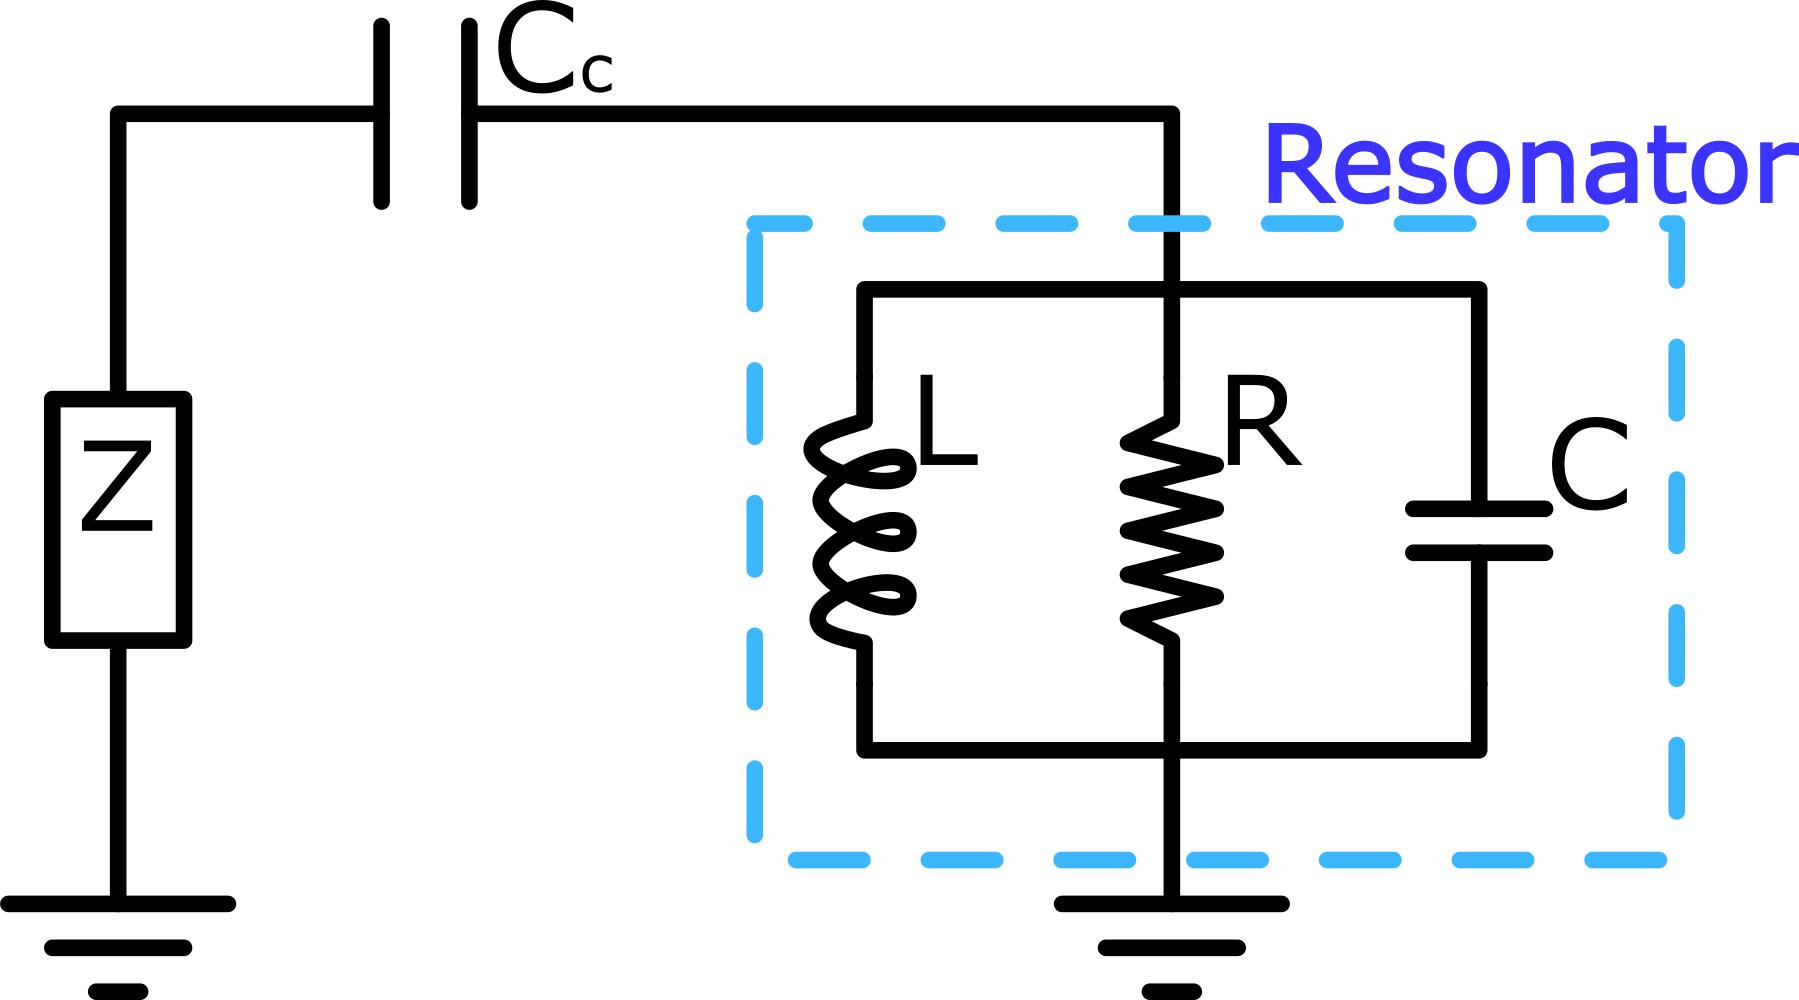
\includegraphics[width=250px]{Figures/external.png}
\decoRule
\caption[External coupling circuit]{The equivalent circuit for the resonator is a parallel RLC circuit.The external losses are in the external inpedence Z of the meaasurement device. The energy in the resonator leaks to the external circuit at a rate $\kappa_e\propto 1/C_c$. The internal losses are due to the resistance R. The rate of instrinsic energy loss in the resonator is $\kappa_i = \kappa - \kappa_e$ where $\kappa$ is the FWHM of the $S_{11}$ response of the resonator.}
\label{fig:external circuit}
\end{figure}

\section{Experiment}

The rectangular cavity used for the experiment is made of aluminium and is shown in Fig.\ref{fig:cavity}.

\begin{figure}
\centering
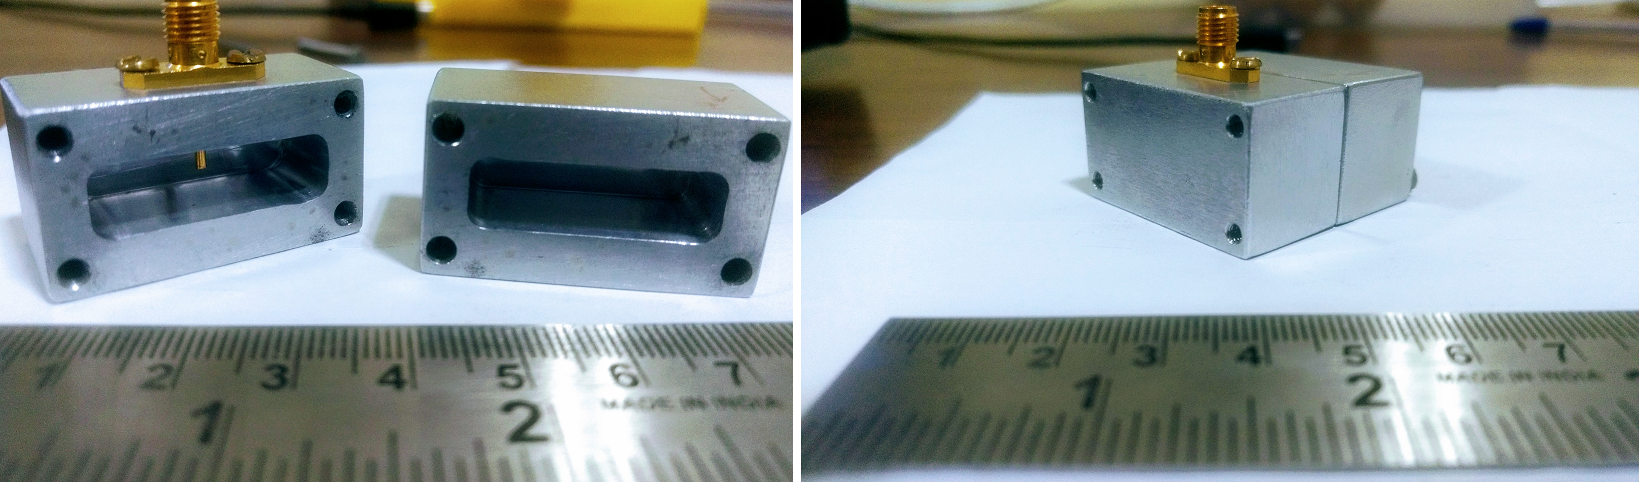
\includegraphics[width=350px]{Figures/cavity.png}
\decoRule
\caption[Aluminium Cavity]{The Aluminium cavity used to make measurements. The dimensions of the hollow in the assembled cavity are $36\times 27\times 8\SI{}{\milli\meter}$. The lengths of the connector pin referred to by Fig.\ref{fig:diff lengths} includes the wall of the cavity.}
\label{fig:cavity}
\end{figure}

The $S_{11}$ parameter is the ratio of the voltage detected to voltage sent into the cavity. It is a complex number with information about the amplitude and phase. It it measured by sending a known signal of a particular frequency with a set amplitude and phase, and detecting the amplitude and phase of the reflected signal after passing through the cavity at the same frequency. A VNA is used to sweep the frequency of the input signal and record the amplitude and phase of the signal returned at the same frequency. The schematic of the circuit used to make measurements at $20mK$ is shown in Fig.\ref{fig:circuit with fridge}. The actual setup of the dilution refrigerator is shown in Fig.\ref{fig:real fridge}.

\begin{figure}
\centering
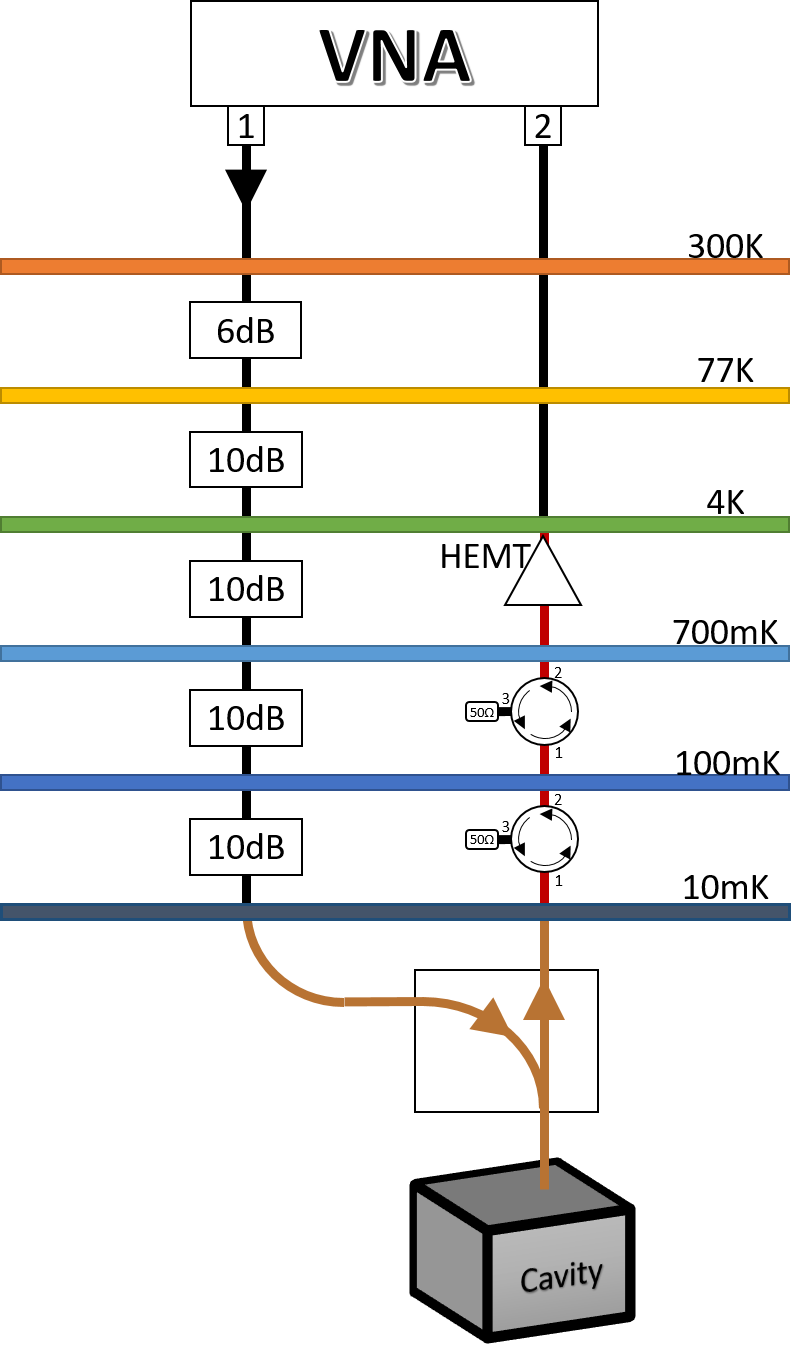
\includegraphics[width=350px]{Figures/circuit.png}
\decoRule
\caption[External Circuit]{The measurement setup for $20mK$ measurements. The input signal is sent from port 1 of the VNA. There are attenuators of appropriate values in between the plates. At the base plate, the input goes into a directional coupler which adds another 20dB attenuation. The output from the cavity is directed towards a HEMT amplifier which is connected to port 2 of the VNA.}
\label{fig:circuit with fridge}
\end{figure}

\begin{figure}
\centering
\includegraphics[width=350px]{Figures/dil_fridge.jpg}
\decoRule
\caption[Dilution Refrigerator]{The Dilution Refrigerator.}
\label{fig:real fridge}
\end{figure}

The $S_{11}$ response for a microwave resonator is given by \cite{Aspelmeyer2014}
\begin{equation}
S_{11}(\omega) = 1-\frac{\kappa_e}{\kappa/2+j(\omega-\omega_0)}
\label{eqn:s11 sym}
\end{equation}
where\\
$\omega_0$ is the resonant frequency of the cavity,\\
$\kappa = \Delta\omega$ is the FWHM of the resonance peak which represents total losses,\\
$\kappa_e$ is the part of $\kappa$ which represents the losses to the external circuit through the capacitor $C_c$.\\
The quality factor can be calculated using $Q = \omega_0/\text{FWHM}$. The internal, external and total quality factors can be calculated using
\begin{align}
Q_{total} &= \frac{\omega_0}{\kappa}\\
Q_{external} &= \frac{\omega_0}{\kappa_e}\\
Q_{internal} &= \left(\frac{1}{Q_{total}}-\frac{1}{Q_{external}}\right)^{-1}\\
\end{align}

The $S_{11}$ response of the cavity is asymmetrical, as shown in Fig. \ref{fig:cavity response}, due to the finite cable length and finite isolation of the directional coupler.
\begin{itemize}
\item The effect of the finite cable length is an added frequency dependent phase factor $\text{exp}(2j\omega l/v_p)$ where $l$ is the cable length and $v_p=c/\sqrt{\epsilon_r}$ is the phase velocity. The '$2$' in the expression is because the cable length is traversed twice.\\
This factor is multiplied to the original expression for $S_{11}$ in \ref{eqn:s11 sym}.
\item The effect of the finite isolation of the directional coupler is modelled by considering a part of the signal as a complex background ($\alpha_i e^{j\phi}$) and the rest of the signal ($(1-\alpha_i)S_{11}$) as the $S_{11}$ response.
\end{itemize}
So the final function used to fit the data from Fig.\ref{fig:circuit with fridge} and get the parameters $\omega_0$,$\kappa$ and $\kappa$ is
\begin{equation}
S_{11}(\omega) = \alpha_i e^{j\phi}+(1-\alpha_i)\left(1-\frac{\kappa_e}{\kappa/2+j(\omega-\omega_0)}\right)e^{2j\omega l/v_p}
\end{equation}

\begin{figure}
\centering
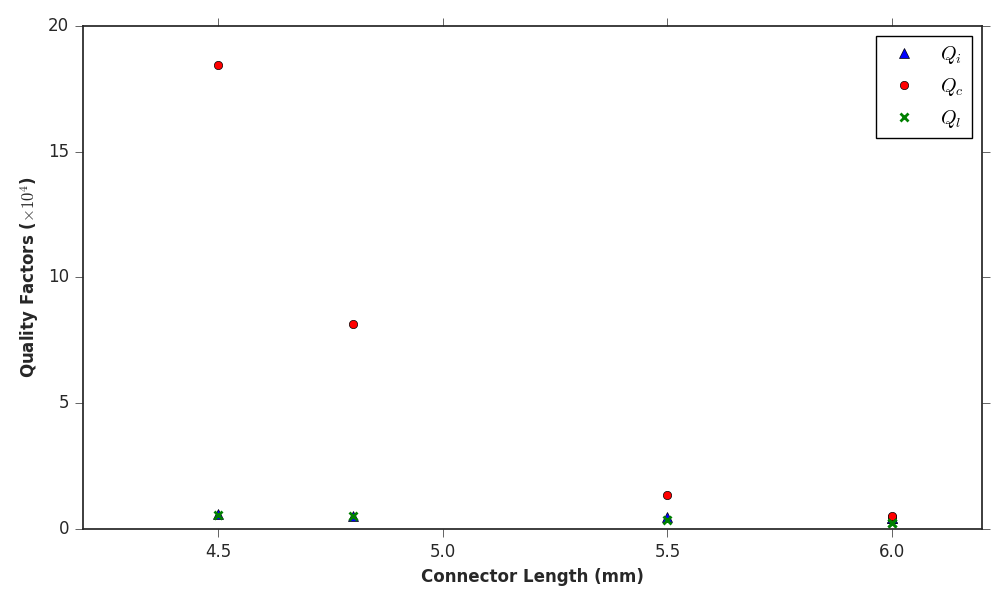
\includegraphics[width=\linewidth]{Figures/diff_lengths.png}
\decoRule
\caption[Quality Factors for different pin lengths]{Quality factors for different pin lengths. $Q_i$ is the internal Quality, $Q_c$ is the external Quality, and $Q_t$ is the total Quality. The coupling Quality Factor $Q_c$ is increasing with decreasing pin lengths.}
\label{fig:diff lengths}
\end{figure}

The $S_{11}$ measurement was performed for different pin lengths\footnote{The lengths of the connector pin referred to here includes the wall of the cavity. So, the actual length of the connector pin that is in the cavity is $\SI{5}{\milli\meter}$ lesser than the given length.} inserted into the cavity at room temperature. The quality factors obtained from this measurement is shown in Fig.\ref{fig:diff lengths}. The coupling Quality Factor $Q_c$ increases with decreasing pin length, while the internal Quality Factor remains the same.

The same measurement is made by using a constant pin length of $4.5 mm$, but this time at a temperature of $20mK$. The internal quality factor is larger than the coupling quality factor at this temperature mainly because aluminium is superconducting below $1.1K$. Fig.\ref{fig:cold qualities} shows a plot of $Q_i$, $Q_c$ and $Q_t$ as a function of the average number of photons in the cavity. A sample plot of amplitude and phase data for a power of -35dBm is shown in Fig.\ref{fig:fit}. The coupling Quality Factor $Q_c$ remains the same, suggesting that it does not depend on the number of photons in the cavity. The internal Quality Factor has an increasing trend. This can be explained using Two-Level Systems in the material which get saturated to their excited states at higher photon numbers\cite{Gao2007}.

\begin{figure}
\centering
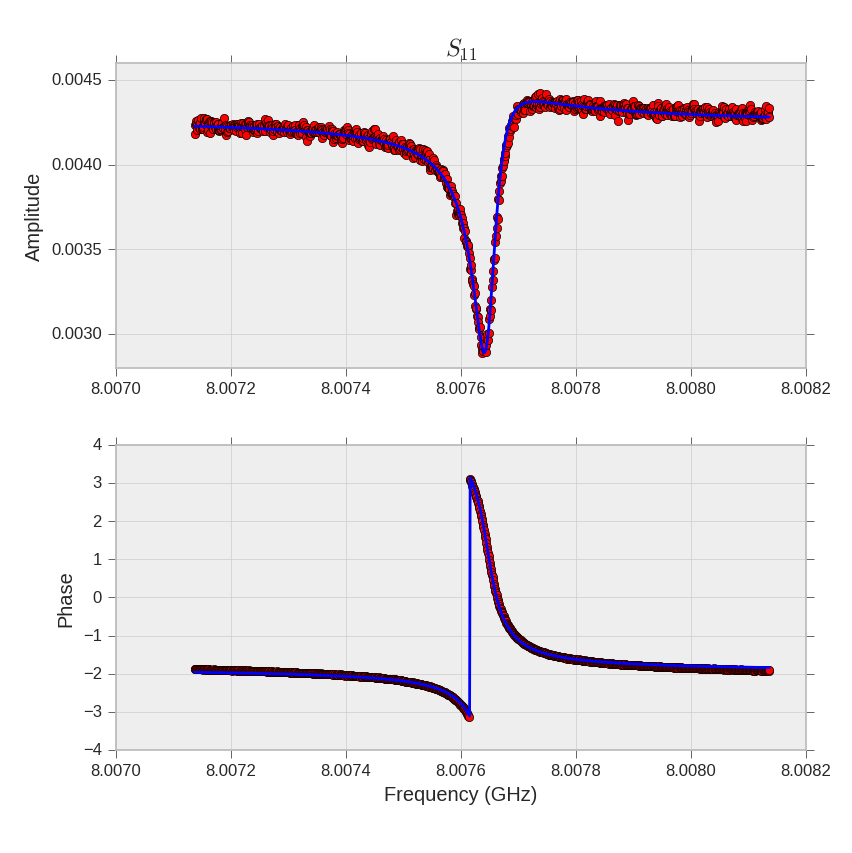
\includegraphics[width=300px]{Figures/s11fit.png}
\decoRule
\caption[Sample $S_{11}$ fit]{A sample of data and fit of $S_{11}$ at 20mK for a power of -35dBm. The red dots are the data from the VNA, and the blue line is the fit.}
\label{fig:fit}
%\end{figure}

%\begin{figure}
\centering
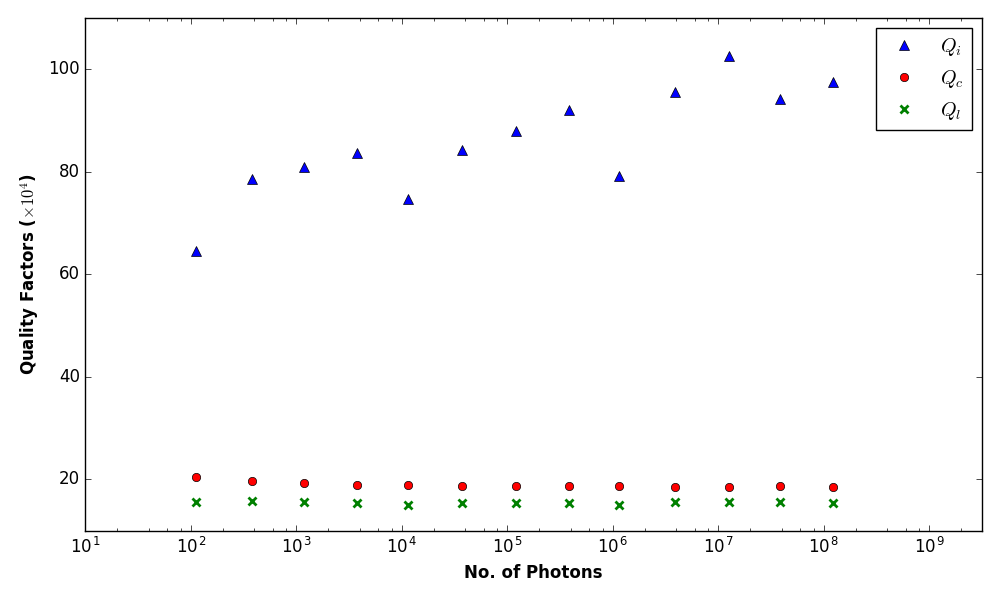
\includegraphics[width=\linewidth]{Figures/cold_qualities.png}
\decoRule
\caption[Quality Factors for different powers at low temperature]{Quality factors for different powers at low temperature. $Q_i$ is the internal Quality, $Q_c$ is the external Quality, and $Q_t$ is the total Quality.}
\label{fig:cold qualities}
\end{figure}